\documentclass[12pt,a4paper]{article}
\usepackage[utf8]{inputenc}
\usepackage[spanish]{babel}
\usepackage{graphicx,color}
\usepackage{amsmath}
\usepackage{amssymb}
\usepackage{amsthm}
\usepackage{cancel}
\usepackage[left=2.5cm,top=2.8cm,bottom=2.6cm,right=2.5cm]{geometry}

\newcommand \tr {\operatorname{Tr}}

\begin{document}

\title{Proyectos MC2}
\author{Cristián G. Sánchez}
	
\maketitle
	
	\section{Dinámica del modelo de espín-bosón}
	La idea del proyecto es estudiar la dinámica del Hamiltoniano
\[\hat{H}=\left(\frac{\hat{p}^2}{2m}+\frac{1}{2}k\hat{q}^2\right)\hat{I}+(a\hat{q}+\epsilon)\hat{\sigma}_z+j\hat{\sigma}_x\]
	que describe un sistema de dos niveles acoplado a un oscilador armónico (los operadores $\hat{\sigma}_i$ son las matrices de Pauli). La dinámica se estudia en la base de productos de un estado del sistema de dos niveles con un estado del oscilador armónico. La base se trunca imponiendo un número máximo de estados del oscilador.
	%Utilizando los parámetros $j=1/10$, $a=1$, $\epsilon=1/4$ y $k=1$, dentro de la aproximación de Born-Oppenheimer (donde $q$ es sólo un parámetro) la diagonalización produce los autovalores que se muestran en la figura:

%\begin{center}	
%	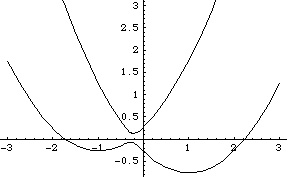
\includegraphics{tlsplot.jpg}
%\end{center}
	Los pasos son:
\begin{enumerate}
	\item Escribir el Hamiltoniano en forma segunda cuantizada.
	\item Calcular los elementos de matriz en la base producto, para un número arbitrario de excitación del oscilador.
	\item Diagonalizar el Hamiltoniano.
	\item Estudiar los autoestados.
	\item Construir el operador evolución a partir de su representación espectral.
	\item Calcular la dinámica a partir de la aplicación del operador evolución a un estado inicial arbitrario.
\end{enumerate}
	Como problemas interesantes se proponen:
	\begin{itemize}
		\item Estudiar la evolución de un paquete de incerteza mínima inicialmente preparado en la superficie del estado electrónico excitado.
		\item Estudiar el espectro a partir de la función de autocorrelación del operador momento dipolar.
	\end{itemize}

\subsection{Una variación}
Una variación de este proyecto puede ser el estudio de los autoestados del sistema de dos niveles acoplado a un número de osciladores armónicos (del orden de 10). Se debe construir una rutina para calcular los elementos de matriz y luego utilizar un método de diagonalización iterativa (método de Lanczos) para obtener los autovalores y autoestados.

\subsection{Otra variación}
Otra variación es agregar otro/s spines, asumirlos fermiones y utilizar segunda cuantización para resolver el problema en 1D acoplando fonones y electrones.

\section{Evolución de paquetes de onda en una dimensión en un potencial arbitrario}
Se propone estudiar la dinámica de un paquete de onda arbitrario en una dimensión en algun potencial externo. Partiendo de la ecuación de Schroedinger dependiente del tiempo
\[
\frac{\partial \psi(x,t)}{\partial t}=-\frac{i}{\hbar}\hat{H}\psi(x,t)
\]
con
\[
\hat{H}=-\frac{\hbar^2}{2m}\frac{\partial^2}{\partial x^2}+V(x).
\]
Discretizando la derivada segunda de la forma
\[
\frac{\partial^2 f(x)}{\partial x^2}=\frac{1}{\delta^2}(f(x-\delta)-2f(x)+f(x+\delta))
\]
se transforma la ecuación diferencial en una ecuación matricial (con variable $x$ discreta) con un operador Hamiltoniano tridiagonal. 

Para integrar la ecuación de movimiento de la función de onda puede utilizarse una expansión de orden $n$ del propagador $\exp\left(\frac{-i}{\hbar}\Delta t\hat{H}\right)$ o el propagador de Crank-Nicholson:
\[
\frac{1-i\hat{H}\Delta t/2}{1+i\hat{H}\Delta t/2}
\]
que tiene la gran ventaja de ser unitario.
Problemas interesantes:
\begin{itemize}
\item Tuneleo de un paquete de incerteza mínima a través de una barrera de potencial.
\item Tuneleo de un paquete a traves de una doble barrera con estados ligados, estudio de la probabilidad de transmisión en función de la energía.
\item Propagación del paquete de incerteza mínima libre, en un potencial armónico y un potencial anarmónico.
\item Agregado de un potencial dependiente del tiempo simulando un campo electromagnético externo.
\item Generalización a dos dimensiones.
\item Agregar un potencial local (armónico por ejemplo), calcular los autoestados y compararlos con los analíticos. Agregar una perturbación (anarmonicidad) y comparar perturbaciones con el resultado computacional.
\item Estudiar la dinámica en respuesta a un potencial externo (para el sistema del ítem anterior) y comprar con perturbaciones dependientes del tiempo.
\item Etc., etc., etc. 
\end{itemize}

\section{Conductancia de una molécula diatómica}
Dado el sistema compuesto por dos hilos monoatómicos conectados a una molécula diatómica:
\begin{center}
	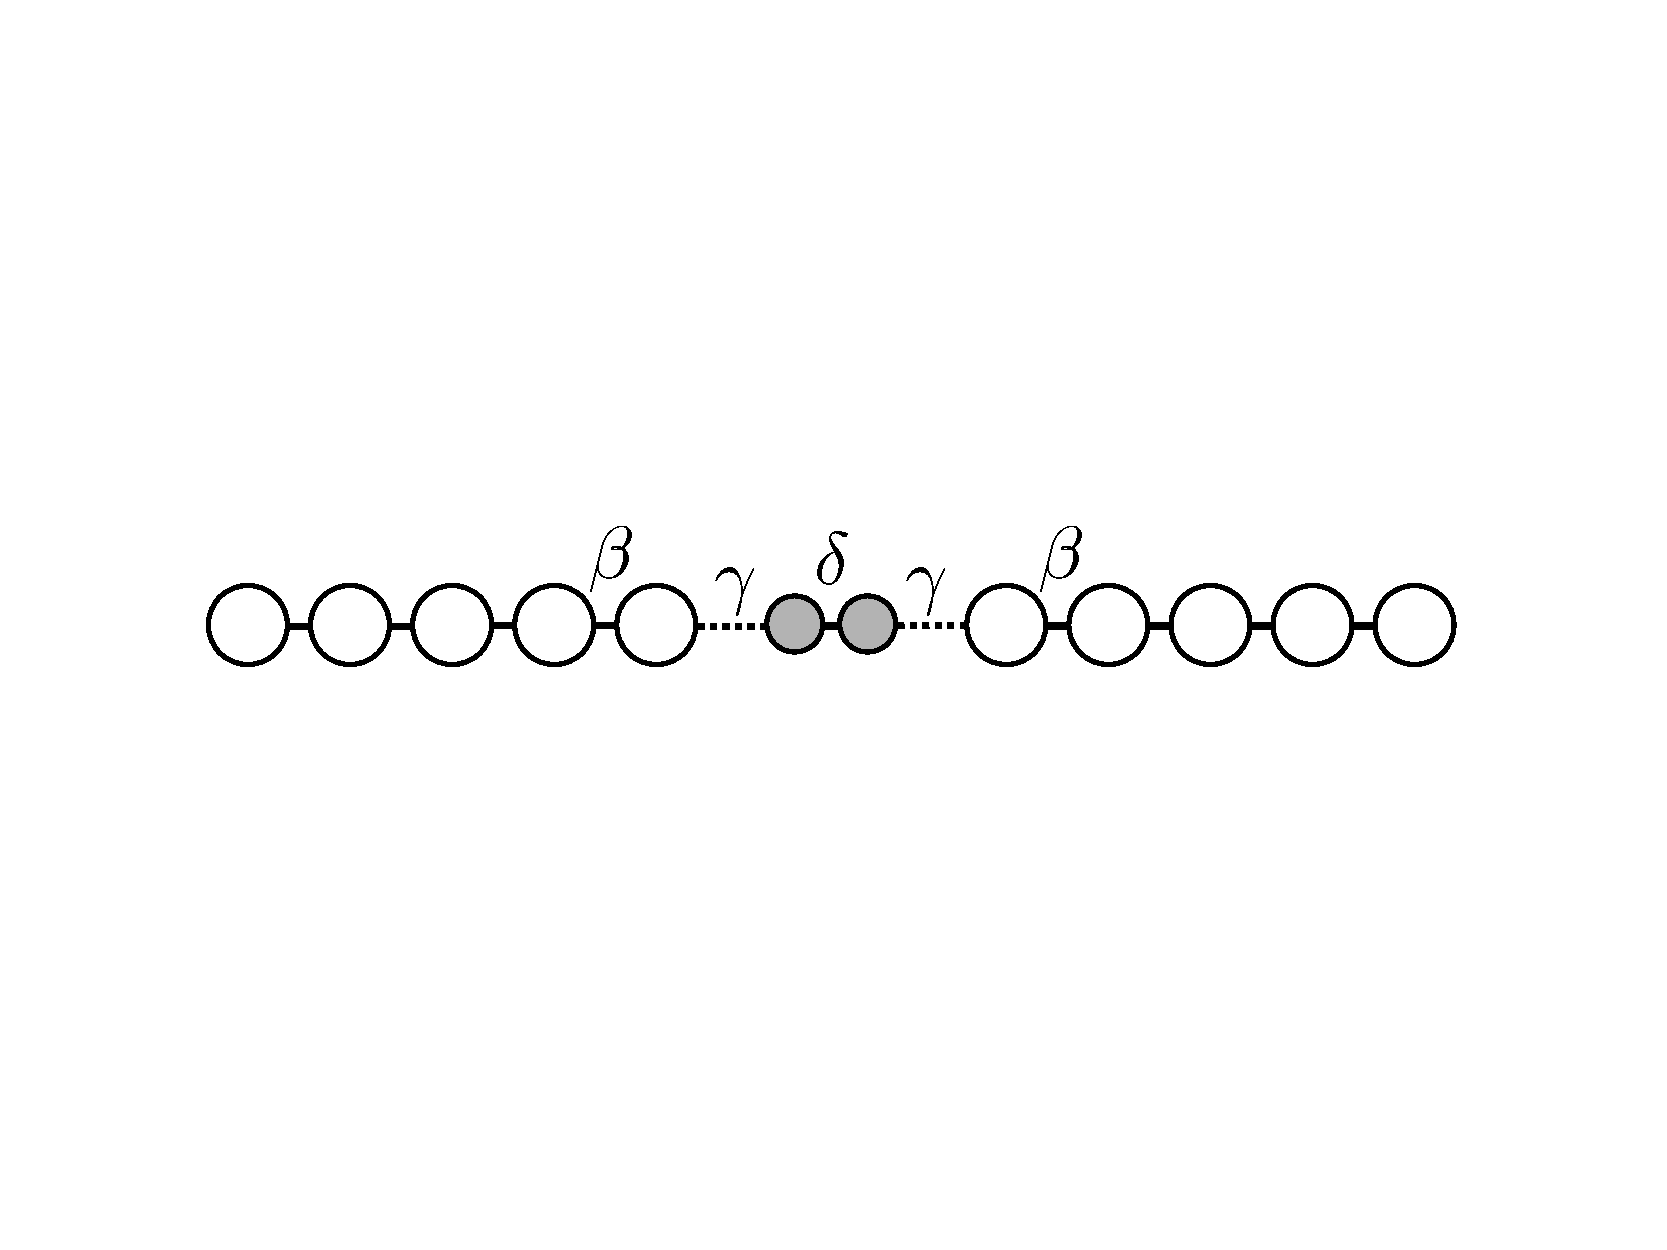
\includegraphics[scale=0.5]{wire.pdf}
\end{center}
Donde el Hamiltoniano posee sólo los elementos de matriz $\beta$ dentro del hilo, $\gamma$ que conecta la molécula con los hilos y $\delta$ entre los átomos de la molécula y cada átomo aporta un único orbital atómico a la base. Los pasos a seguir son:
\begin{itemize}
	\item Diagonalizar el Hamiltoniano en presencia de un campo externo que ocasione cargado de uno de los hilos, esto es, un potencial constante $-V/2$ al electrodo izquierdo y un potencial $V/2$ al lado derecho.
	\item Utilizando los autovalores $\epsilon_i$ y los autoestados $\psi_i$ Construir la matriz densidad de un cuerpo
	\[\hat{\rho}=\sum_i |\psi_i\rangle f(\epsilon_i-\mu) \langle\psi_i|\]
	en la base donde $f(\epsilon_i-\mu)$ es la función de Fermi y $\mu$ el nivel de fermi.
	\item Remover el potencial externo e integrar la ecuación de movimiento de la matriz densidad $\dot{\rho}=-\frac{i}{\hbar}[\hat{H},\rho]$ con el algoritmo:
	$\rho(t+\Delta t)=\dot{\rho}(t)+2 \Delta t \rho(t-)$
	\item Calcular la corriente que atraviesa la molécula en función del tiempo.
	\item Construir el espectro de conductancia de la molécula a partir de la corriente de estado estacionario en función de la diferencia de potencial aplicado y comparar con el resultado obtenido de la formulación de Landauer.
\end{itemize}


\section{Dinámica del sistema de dos niveles acoplado a un campo oscilante}

Dado el Hamiltoniano no perturbado siguiente
\begin{equation}
\hat{H}^0 = \left[\begin{array}{cc}
\epsilon_1 & \beta \\ 
\beta & \epsilon_2
\end{array}\right]
\end{equation}
correspondiente a un sistema de dos niveles, y el operador momento dipolar
\begin{equation}
\hat{\mu}\right = \left[\begin{array}{cc}
-\delta & 0 \\ 
0 & \delta
\end{array}\right]
\end{equation}
\begin{itemize}
\item Diagonalizando el Hamiltoniano perturbado $\hat{H}=\hat{H}^0+E\hat{\mu}$, calcule numéricamente la polarizabilidad estática $\frac{\partial\langle\mu\rangle}{\partial E}$ en función de $\beta$.
\item Escriba un programa que permita integrar la ecuación de Liouville con el camiltoniano perturbado $\hat{H}=\hat{H}^0+f(t)\hat{\mu}$, donde $f(t)$ es una función del tiempo, para un estado inicial arbitrario. Utilice el siguiente algoritmo $\hat{\rho}(t+\Delta t) = \hat{\rho}(t-\Delta t) + 2\Delta t \frac{\partial\hat{\rho}}{\partial t}$. 
\item Dado un sistema preparado en el estado $|1\rangle$ Analice el comportamiento de los elementos diagonales de $\rho$. Calcule la evolución del momento dipolar en función del tiempo cuando $f(t)=0$. 
\item Sea $f(t)=\sin(\omega  t)$. Integre la ecuación de Liouville y determine la evolución del momento dipolar con el tiempo. Determine la evolución de la energía del sistema. Calcule la potencia media absorbida (sobre un período de oscilación) en función de $\omega$. Calcule la potencia media a partir de su ecuación de movimiento.
\item Estudie cómo responde la energía a la acción de pulsos gausianos $f(t)=e^-(t-t_0)^2/\sigma^2 \sin(\omega t)$. Encuentre la forma del pulso que lleva al sistema del estado fundamental al estado excitado. Qué ocurre cuando se aplica este pulso a un sistema preparado en el estado excitado?
\item Compare el cálculo numérico con resultados de teoría dde pertirbaciones para el caso de campo estático y dependiente del tiempo.

%\section{Integrales de camino en tiempo imaginario}
%
%Este proyecto esta un poco más crudo que los otros ya que personalmente no lo he hecho nunca! La idea sería utilizar path integral molecular dynamics para estudiar un sistema de una partícula en un potencial externo. Una descripción detallada de lo involucrado puede leerse en {\tt http://www.fz-jülich.de/nic-series/volume10/volume10.html} (ver los dos capitulos de Mark Tuckerman). 







\end{document}
